\documentclass[ngerman,compress,hyperref={bookmarks}]{beamer}
\usetheme{Antibes}
\useoutertheme{infolines}
\usepackage[utf8x]{inputenc}

\usepackage{multirow}

\usepackage{colortbl}
\definecolor{dunkelgrau}{rgb}{0.8, 0.8, 0.8}

\usepackage{wasysym}

\logo{
\includegraphics[height=1cm]{images/logoHAW}}
\usepackage{graphicx}
%\usepackage[%
%	bibstyle=authoryear,%
%	citestyle=authoryear,%
%	bibencoding=utf8,%
%	bibtex8=true,%
%	sorting=nyt,%
%	sortcites=true,%
%	maxnames=2,%
%	babel=other,%
%	block=space,%
%	backref=false,%
%	natbib=true,%
%	hyperref=true,%
%]{biblatex}
%\bibhang1em
%\usepackage[style=authortitle-icomp]{biblatex}
%\bibliography{routing_atlas}

%\setbeamertemplate{bibliography entry title}{}
%\setbeamertemplate{bibliography entry location}{}

\title{Erweiterung des Routing-Atlas}
\subtitle{Vortrag: Anwendung 2\\ Related Work}
\subject{Routing-Atlas, Topology}
\author{Andreas Krohn}
\institute[HAW]{Hochschule für Angewandte Wissenschaften Hamburg}
\date[SoSe 2012]{26. April 2012}

\begin{document}
\frame[plain]{\titlepage}

\section*{Agenda}
\begin{frame}{Agenda} \setcounter{tocdepth}{1} \tableofcontents[part=1] \setcounter{tocdepth}{3} \end{frame}

\part{Hauptteil}
\section{Rückblick}

\subsection{Was ist der Routing-Atlas?}
\begin{frame}{Was ist der Routing-Atlas?}
  \begin{itemize}
    \item Projekt der inet AG und des BSI
    \item Topologieanalyse um landesspezifische Teile des Internets zu
    \begin{enumerate}
      \item Identifizieren
      \item Klassifizieren
      \item Visualisieren
    \end{enumerate}
  \end{itemize}
  \vspace{1cm}
  \begin{thebibliography}{}
    \bibitem{schmidt2010} ``Ein Routing-Atlas für die strukturelle und visuelle Exposition des deutschen Internets''
    \newblock Thomas C. Schmidt, Matthias Wählisch, Markus de Brün und Thomas Häberlen (2010)\\[-20pt]
  \end{thebibliography}
\end{frame}

\subsection{Bestandteile des Routingatlas}
\begin{frame}{Bestandteile des Routingatlas}
  \begin{enumerate}
  \item Identifikation deutscher Autonomer Systeme
  \begin {itemize}
    \item IP-Blöcke identifizieren
    \item Zu IP-Präfixen auflösen
    \item IP-Päfixe Autonomen Systemen zuordnen
  \end{itemize}
  \item Neu dazugekommen: Validierung mittels Maxmind \& Cymru
  \item Klassifikation Autonomer Systeme
  \begin{itemize}
    \item Topologische Einordnung
    \item Branchen
  \end{itemize}
  \item Routing-Graphen bilden
  \begin{itemize}
    \item shortest path matrix des NEC-Lab
  \end{itemize}
  \item Visualisierung der (Teil)Graphen
  \end{enumerate}
\end{frame}

\subsection{Ziel}
%\begin{frame}<1-2>{Ziel}
\begin{frame}{Ziel}
  \begin{center}
    {\Large Erweiterung des Routing-Atlas}\\
    \vspace{0.5cm}
    shortest path matrix ersetzen\\
    \vspace{0.5cm}
    Dazu:
    \begin{itemize}
      \item Datenquellen (Routingtabellen, BGP Peering Informationen der IRR)
      %\item \only<1>{Heuristik zur Bewertung von Inter-AS Links}\only<2>{\textbf{Heuristik zur Bewertung von Inter-AS Links}}
      \item Heuristik zur Bewertung von Inter-AS Links
      %\item \only<1>{Kürzeste Wege berechnen}\only<2>{\textbf{Kürzeste Wege berechnen}}
      \item Kürzeste Wege berechnen
    \end{itemize}
  \end{center}
\end{frame}

\section*{Agenda}
\begin{frame}{Agenda} \setcounter{tocdepth}{1} \tableofcontents[part=1] \setcounter{tocdepth}{3} \end{frame}

\section{Begriffe, Grundlagen}
\begin{frame}{Begiffe, Grundlagen}
  \begin{columns}[c]
    \begin{column}{0.75\textwidth}
      \begin{itemize}
        \item Internet: Ansammlung Autonomer Systeme (ASe)
        \item Geschäftsbeziehung zwischen ASen $\rightarrow$ AS Link
      \end{itemize}
      \begin{description}
        \item[C2P] \textbf{C}ustomer bezahlt \textbf{P}rovider für Transit
        \item[PP] \textbf{P}eer-\textbf{P}eer - kostenneutralen Austausch von Traffic
      \end{description}
      \begin{itemize}
        \item Öffentlich verfügbar: BGP dumps, traceroutes, looking glass server
        \item \textbf{Aber} keine zentrale Verwaltung, Vermessungsanstalt, "Ground truth"
      \end{itemize}
      ......... \\
      kl. Grafik?
    \end{column}
  \end{columns}
\end{frame}

%\section{AS-Beziehungen, valley-free routing}
%\begin{frame}{AS-Beziehungen, valley-free routing}
% \begin{columns}[c]
%  \begin{column}{0.2\textwidth}
%  \end{column}
%  \begin{column}{0.5\textwidth}
%    \begin{enumerate}
%     \item[customer-provier] customer zahlt für Transit
%     \item[peering] kostenloser Trafficaustausch
%     \item[sibling] kostenloser Transit\\ \vspace{0.5cm}
%     \item[valley-free routing] Transit nur über ``höhere'' ASes
%    \end{enumerate}
%  \end{column}
%  \begin{column}{0.3\textwidth}
%   \begin{figure}
%    \label{asrelations}
%    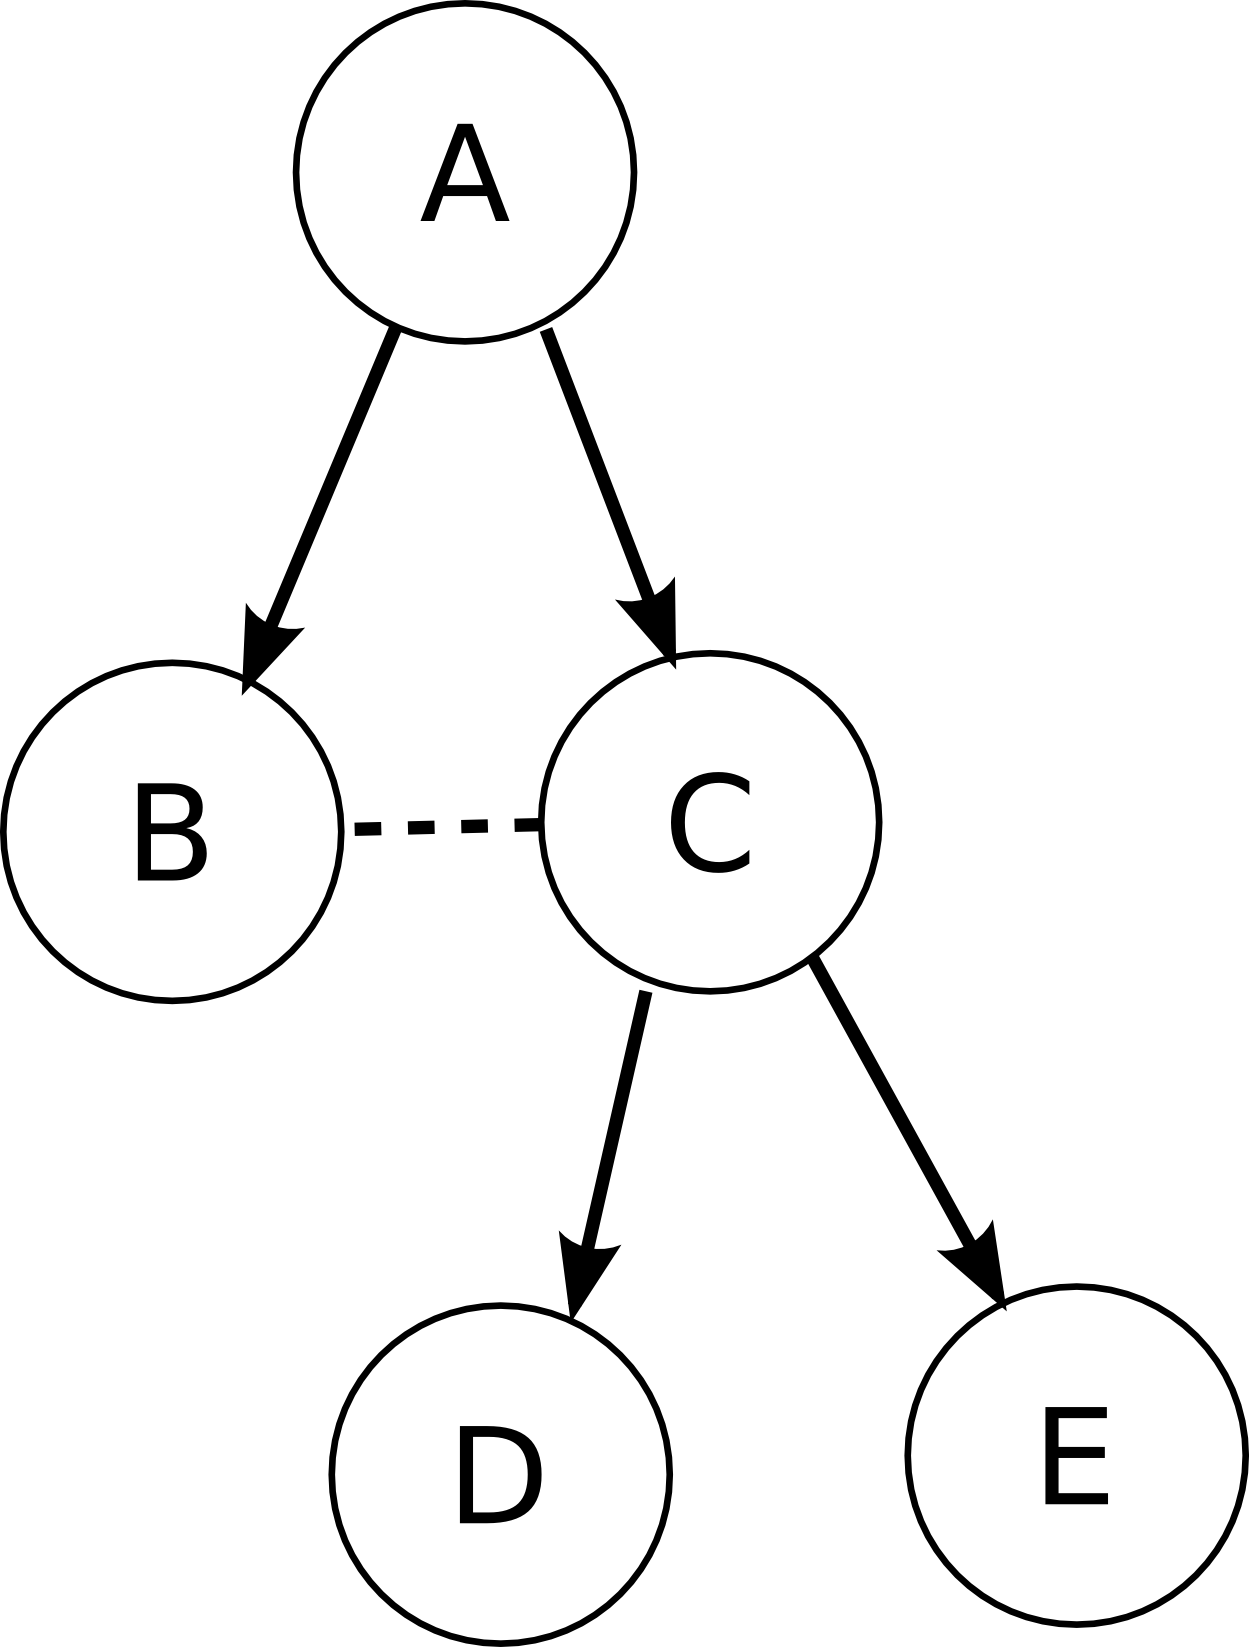
\includegraphics[width=1\textwidth]{images/asrelation}
%   \end{figure}
%    {\scriptsize }
%  \end{column}
% \end{columns}
%\end{frame}


\section{Related Work}

\subsection{Topologiemodellierung}

\begin{frame}{On power-law relationships of the Internet topology}{1999}
  \begin{columns}[c]
    \begin{column}{0.5\textwidth}
      \begin{itemize}
        \item \cite{Faloutsos:1999:PRI:316194.316229}
        \item Graphentheoretische Betrachtung der Inter- \& Intradomain Topologie
        \item Entdeckung exponentieller Verhältnisse zwischen ..
      \end{itemize}
    \end{column}
    \begin{column}{0.1\textwidth}
      \begin{figure}
        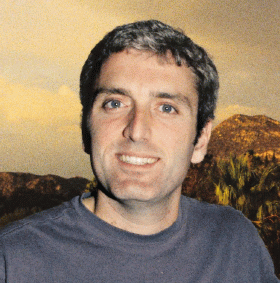
\includegraphics[width=1\textwidth]{images/faloutsos_m}\\
        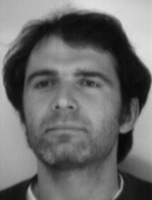
\includegraphics[width=1\textwidth]{images/faloutsos_p}\\
        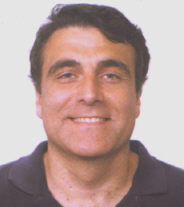
\includegraphics[width=1\textwidth]{images/faloutsos_c}
        \label{faloutsos}
      \end{figure}
    \end{column}
    \begin{column}{0.3\textwidth}
      {\scriptsize Micalis Faloutsos\\
      \vspace{0.1cm}
      University of California\\
      \vspace{0.8cm}
      Petros Faloutsos\\
      \vspace{0.1cm}
      University of Toronto\\
      \vspace{0.7cm}
      Christos Faloutsos\\
      \vspace{0.1cm}
      Carnegie Mellon University}
    \end{column}
  \end{columns}
\end{frame}

\begin{frame}{On Inferring Autonomous System Relationships in the Internet}{2001}
\begin{columns}[c]
 \begin{column}{0.5\textwidth}
  \begin{itemize}
   \item \cite{Gao:2001:IAS:504611.504616}
   \item AS Pfade aus BGP Routing Tabellen
   \item Knotengrad als Heuristik
   \item Einordnung in customer-provider/peering/sibling
  \end{itemize}
 \end{column}
 \begin{column}{0.1\textwidth}
  \begin{figure}
   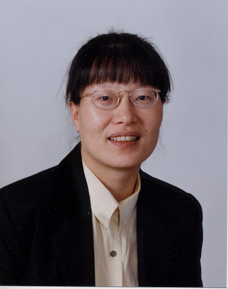
\includegraphics[width=1\textwidth]{images/gao}
   \label{gao}
  \end{figure}
 \end{column}
 \begin{column}{0.3\textwidth}
  {\scriptsize Lixin Gao\\
  \vspace{0.1cm}
  University of Massachusetts\\
  AT\&T Research Labs}
 \end{column}
\end{columns}
\end{frame}

\begin{frame}{Type of Relationship (ToR)}
 \begin{columns}[c]
  \begin{column}{0.5\textwidth}
   \begin{itemize}
    \item \cite{Subramanian:2001:CIH:894120, Di_Battista:2007:CTR:1279660.1279662}
    \item ``Sichtweisen'' getrennt betrachten
    \item Graphentheoretisches Problem:
    \begin{itemize}
     \item Kanten als \emph{uphill}, \emph{downhill} oder \emph{peering} markieren
     \item Dabei valide Pfade erreichen
    \end{itemize}
    \item (Stark) NP-vollständig
    \item Heuristik: AS Rank
   \end{itemize}

  \end{column}
  \begin{column}{0.1\textwidth}

  \end{column}
  \begin{column}{0.3\textwidth}

  \end{column}
 \end{columns}

\end{frame}


\begin{frame}{Collection the Internet AS-level Topology}{2005}
\begin{columns}[c]
 \begin{column}{0.5\textwidth}
  \begin{itemize}
   \item \cite{Zhang:2005:CIA:1052812.1052825}
   \item ``most complete AS-level topology''
   \item route servers, looking glasses, routing registries
   \item routing updates
  \end{itemize}
 \end{column}
 \begin{column}{0.08\textwidth}
  \begin{figure}
   \label{zhang_et_al}
   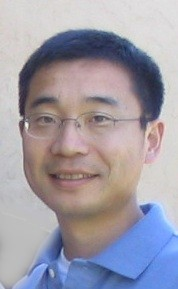
\includegraphics[width=1\textwidth]{images/zhang_b}\\
   
\includegraphics[width=1\textwidth]{images/person}\\
   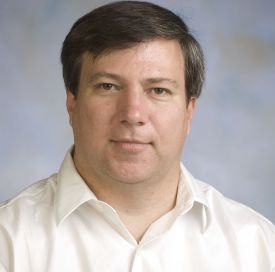
\includegraphics[width=1\textwidth]{images/massey}\\
   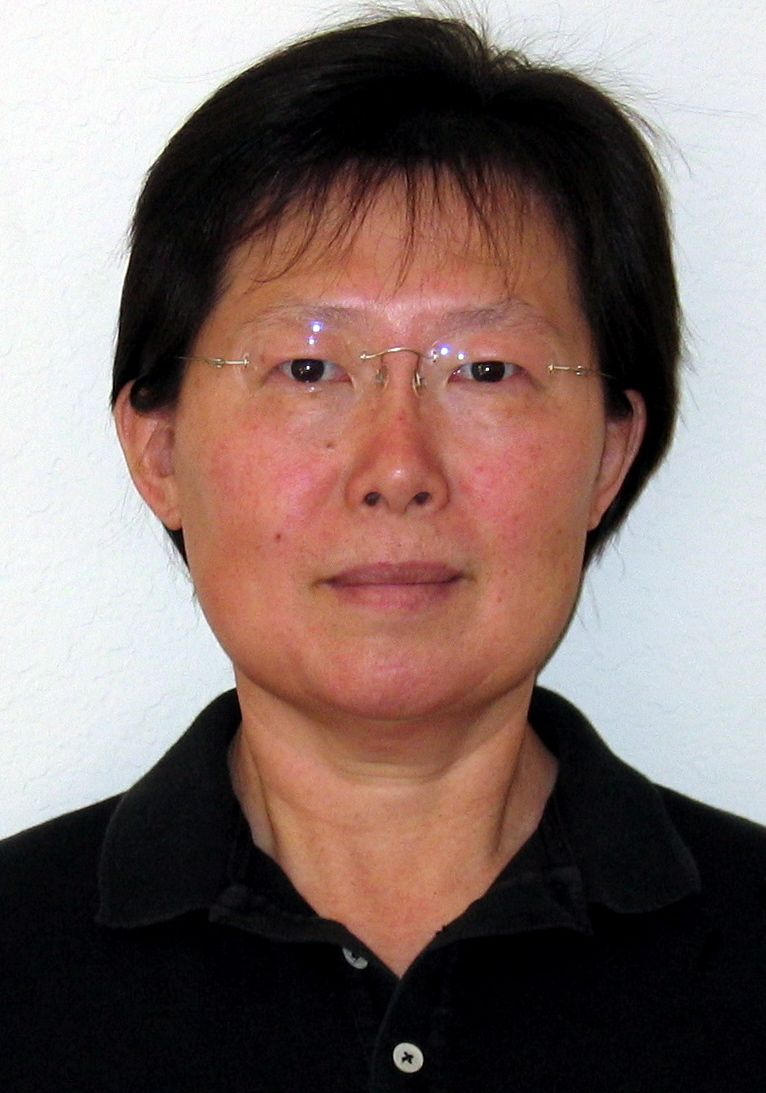
\includegraphics[width=1\textwidth]{images/zhang_l}
  \end{figure}
 \end{column}
 \begin{column}{0.3\textwidth}
  {\scriptsize Beichuan Zhang\\
  \vspace{0.1cm}
  UCLA\\
\vspace{0.7cm}
  Raymond Liu\\
\vspace{0.1cm}
UCLA\\
\vspace{0.3cm}
  Daniel Massey\\
\vspace{0.1cm}
  Colorado State University\\
\vspace{0.3cm}
  Lixia Zhang\\
\vspace{0.1cm}
  UCLA}
 \end{column}
\end{columns}
\end{frame}


\section*{Agenda}
\begin{frame}{Agenda} \setcounter{tocdepth}{1} \tableofcontents[part=1] \setcounter{tocdepth}{3} \end{frame}

\section{Ausblick}
\begin{frame}{Ausblick}
\begin{itemize}
 \item Aktuelle shortest path matrix
 \begin{itemize}
  \item Topologieänderungen
 \end{itemize}\vspace{1cm}
 \item Andere Länder, Visualisierungen, Online-Tool, IPv6
 \begin{itemize}
  \item Breiteres Publikum
  \item Zukunftsfähigkeit
 \end{itemize}
\end{itemize}
\end{frame}

\part{Ende}
%\section{kthxbye}
\begin{frame}{Ende}
\begin{columns}[t]
\begin{column}{0.5\textwidth}
 \begin{center}
 \vspace{1cm}
 Vielen Dank für die Aufmerksamkeit\\
 \vspace{1.5cm}
 Fragen\ldots?
 \end{center}
\end{column}
\begin{column}{0.5\textwidth}
 \vspace{-1cm}
 \begin{figure}
  \label{asngraph_all}
%  \includegraphics[width=\textwidth]{asgraph_catall-pos-betweenness}
%  \caption{AS-Graph (gesamt DE)}
 \end{figure}
\end{column}
\end{columns}
\end{frame}

\section{Literatur}
\begin{frame}[plain]{Literatur}
\scriptsize
\bibliographystyle{alpha}
\bibliography{folien}
% \begin{thebibliography}{}
% \bibitem{schmidt2010} ``Ein Routing-Atlas für die strukturelle und visuelle Exposition des deutschen Internets''
% \newblock Thomas C. Schmidt, Matthias Wählisch, Markus de Brün und Thomas Häberlen (2010)\\[-20pt]
% \bibitem{waehlisch2010-1} ``Towards a Nation-Centric Understanding of the Internet''
% \newblock Matthias Wählisch, Thomas C. Schmidt, Sebastian Meiling, Markus de Brün, Thomas Häberlen (2010) Proc. of the ACM SIGCOMM CoNEXT. Student Workshop\\[-20pt]
% \bibitem{waehlisch2010-2} ``A Framework for Nation-Centric Classification and Observation of the Internet''
% \newblock Matthias Wählisch, Sebastian Meiling, Thomas C. Schmidt (2010) Proc. of the ACM SIGCOMM CoNEXT. Student Workshop\\[-20pt]
% \bibitem{winter2009} ``Modeling the Internet Routing Topology - in less than 24h''
% \newblock Rolf Winter (2009) Proc. of the 2009 ACM/IEEE/SCS 23rd Workshop on Principles of Advanced and Distributed Simulation, pp. 72-79\\[-20pt]
% \bibitem{karlin2009} ``Nation-State Routing: Censorship, Wiretapping, and BGP''
% \newblock Josh Karlin, Sephanie Forrest and Jennifer Rexford (2009) arXiv.org/CoRR, \url{http://arXiv.org/abs/0903.3218}\\[-20pt]
% %\setbeamertemplate{bibliography item}[book]\bibitem{turau2009} ``Algorithmische Graphentheorie''
% %\newblock Volker Turau (2009) München/Oldenbourg Wissenschaftsverlag GmbH\\[-20pt]\setbeamertemplate{bibliography item}[default]
% \bibitem{zhang2005} ``Collecting the AS-level Topology''
% \newblock Beichuan Zhang, Raymond Liu, Daniel Massey and Lixia Zhang (2005) ACM SIGCOMM Computer Communication Review, vol. 35, no. 1, pp.53-61\\[-20pt]
% \bibitem{gao2001} ``On Inferring Autonomous System Relationships in the Internet''
% \newblock Lixin Gao (2001) IEEE/ACM Transactions on Networking, vol. 9, number. 6, pp. 733-745\\[-20pt]
% \setbeamertemplate{bibliotraphy item}[triangle]\bibitem{pritlove2010} ``Die Internetwolke''
% \newblock Tim Pritlove, Elisa Jasinska und Christian Kaufmann (2010) \url{http://chaosradio.ccc.de/cre144.html}
% \end{thebibliography}
\end{frame}

\section{Bildquellen}
\begin{frame}[plain]{Bilderquellen}
  %\scriptsize
  \tiny
  \begin{table}
    \begin{tabular}{ c p{0.8\textwidth} }
      Seite & Quelle \\ \hline
      & \multirow{3}{0.8\textwidth}{\url{http://www.cs.ucr.edu/~michalis/},\\ \url{http://www.cse.yorku.ca/cspeople/faculty/pfal/index.html},\\ \url{http://www.cs.cmu.edu/~christos/}} \\
      \pageref{faloutsos}& \\
      & \\ \hline
      \pageref{gao} & \url{http://www-unix.ecs.umass.edu/~lgao/} \\ \hline
      & \multirow{3}{0.8\textwidth}{\url{http://www.cs.arizona.edu/~bzhang/},\\ \url{http://www.cs.colostate.edu/~massey/},\\ \url{http://www.cs.ucla.edu/~lixia/}} \\
      \pageref{zhang_et_al} & \\
      & \\
      \hline
    \end{tabular}
  \end{table}
\end{frame}

\end{document}
